\documentclass{ximera}

\title{Pre-Requisites}
%%%% List of skills:
%    Arithmetic with fractions and (up to) three digit numbers without using a calculator.
%    Isolating a variable in a multivariable linear equality.
%    Correctly distributing expressions and combining like terms.
%    Interval notation.
%    Graphing points on an x-y plane, and writing the coordinates of the points on an x-y plane.
%    Order of Operations.
%    Fraction Vocabulary and fluency.

\usepackage{longdivision}
\usepackage{polynom}
\usepackage{float}% Use `H' as the figure optional argument to force it's vertical placement to conform to source.
%\usepackage{caption}% Allows us to describe the figures without having "figure 1:" in it. :: Apparently Caption isn't supported.
%    \captionsetup{labelformat=empty}% Actually does the figure configuration stated above.
\usetikzlibrary{arrows.meta,arrows}% Allow nicer arrow heads for tikz.
\usepackage{gensymb, pgfplots}
\usepackage{tabularx}
\usepackage{arydshln}
\usepackage[margin=1.5cm]{geometry}
\usepackage{indentfirst}

\setlength\parindent{16pt}

\graphicspath{
  {./}
  {./explorePolynomials/}
  {./exploreRadicals/}
  {./graphing/}
}

%% Default style for tikZ
\pgfplotsset{my style/.append style={axis x line=middle, axis y line=
middle, xlabel={$x$}, ylabel={$y$}, axis equal }}


%% Because log being natural log is too hard for people.
\let\logOld\log% Keep the old \log definition, just in case we need it.
\renewcommand{\log}{\ln}


%%% Changes in polynom to show the zero coefficient terms
\makeatletter
\def\pld@CF@loop#1+{%
    \ifx\relax#1\else
        \begingroup
          \pld@AccuSetX11%
          \def\pld@frac{{}{}}\let\pld@symbols\@empty\let\pld@vars\@empty
          \pld@false
          #1%
          \let\pld@temp\@empty
          \pld@AccuIfOne{}{\pld@AccuGet\pld@temp
                            \edef\pld@temp{\noexpand\pld@R\pld@temp}}%
           \pld@if \pld@Extend\pld@temp{\expandafter\pld@F\pld@frac}\fi
           \expandafter\pld@CF@loop@\pld@symbols\relax\@empty
           \expandafter\pld@CF@loop@\pld@vars\relax\@empty
           \ifx\@empty\pld@temp
               \def\pld@temp{\pld@R11}%
           \fi
          \global\let\@gtempa\pld@temp
        \endgroup
        \ifx\@empty\@gtempa\else
            \pld@ExtendPoly\pld@tempoly\@gtempa
        \fi
        \expandafter\pld@CF@loop
    \fi}
\def\pld@CMAddToTempoly{%
    \pld@AccuGet\pld@temp\edef\pld@temp{\noexpand\pld@R\pld@temp}%
    \pld@CondenseMonomials\pld@false\pld@symbols
    \ifx\pld@symbols\@empty \else
        \pld@ExtendPoly\pld@temp\pld@symbols
    \fi
    \ifx\pld@temp\@empty \else
        \pld@if
            \expandafter\pld@IfSum\expandafter{\pld@temp}%
                {\expandafter\def\expandafter\pld@temp\expandafter
                    {\expandafter\pld@F\expandafter{\pld@temp}{}}}%
                {}%
        \fi
        \pld@ExtendPoly\pld@tempoly\pld@temp
        \pld@Extend\pld@tempoly{\pld@monom}%
    \fi}
\makeatother




%%%%% Code for making prime factor trees for numbers, taken from user Qrrbrbirlbel at: https://tex.stackexchange.com/questions/131689/how-to-automatically-draw-tree-diagram-of-prime-factorization-with-latex

\usepackage{forest,mathtools,siunitx}
\makeatletter
\def\ifNum#1{\ifnum#1\relax
  \expandafter\pgfutil@firstoftwo\else
  \expandafter\pgfutil@secondoftwo\fi}
\forestset{
  num content/.style={
    delay={
      content/.expanded={\noexpand\num{\forestoption{content}}}}},
  pt@prime/.style={draw, circle},
  pt@start/.style={},
  pt@normal/.style={},
  start primeTree/.style={%
    /utils/exec=%
      % \pt@start holds the current minimum factor, we'll start with 2
      \def\pt@start{2}%
      % \pt@result will hold the to-be-typeset factorization, we'll start with
      % \pgfutil@gobble since we don't want a initial \times
      \let\pt@result\pgfutil@gobble
      % \pt@start@cnt holds the number of ^factors for the current factor
      \def\pt@start@cnt{0}%
      % \pt@lStart will later hold "l"ast factor used
      \let\pt@lStart\pgfutil@empty,
    alias=pt-start,
    pt@start/.try,
    delay={content/.expanded={$\noexpand\num{\forestove{content}}
                            \noexpand\mathrlap{{}= \noexpand\pt@result}$}},
    primeTree},
  primeTree/.code=%
    % take the content of the node and save it in the count
    \c@pgf@counta\forestove{content}\relax
    % if it's 2 we're already finished with the factorization
    \ifNum{\c@pgf@counta=2}{%
      % add the factor
      \pt@addfactor{2}%
      % finalize the factorization of the result
      \pt@addfactor{}%
      % and set the style to the prime style
      \forestset{pt@prime/.try}%
    }{%
      % this simply calculates content/2 and saves it in \pt@end
      % this is later used for an early break of the recursion since no factor
      % can be greater then content/2 (for integers of course)
      \edef\pt@content{\the\c@pgf@counta}%
      \divide\c@pgf@counta2\relax
      \advance\c@pgf@counta1\relax % to be on the safe side
      \edef\pt@end{\the\c@pgf@counta}%
      \pt@do}}

%%% our main "function"
\def\pt@do{%
  % let's test if the current factor is already greather then the max factor
  \ifNum{\pt@end<\pt@start}{%
    % great, we're finished, the same as above
    \expandafter\pt@addfactor\expandafter{\pt@content}%
    \pt@addfactor{}%
    \def\pt@next{\forestset{pt@prime/.try}}%
  }{%
    % this calculates int(content/factor)*factor
    % if factor is a factor of content (without remainder), the result will
    % equal content. The int(content/factor) is saved in \pgf@temp.
    \c@pgf@counta\pt@content\relax
    \divide\c@pgf@counta\pt@start\relax
    \edef\pgf@temp{\the\c@pgf@counta}%
    \multiply\c@pgf@counta\pt@start\relax
    \ifNum{\the\c@pgf@counta=\pt@content}{%
      % yeah, we found a factor, add it to the result and ...
      \expandafter\pt@addfactor\expandafter{\pt@start}%
      % ... add the factor as the first child with style pt@prime
      % and the result of int(content/factor) as another child.
      \edef\pt@next{\noexpand\forestset{%
        append={[\pt@start, pt@prime/.try]},
        append={[\pgf@temp, pt@normal/.try]},
        % forest is complex, this makes sure that for the second child, the
        % primeTree style is not executed too early (there must be a better way).
        delay={
          for descendants={
            delay={if n'=1{primeTree, num content}{}}}}}}%
    }{%
      % Alright this is not a factor, let's get the next factor
      \ifNum{\pt@start=2}{%
        % if the previous factor was 2, the next one will be 3
        \def\pt@start{3}%
      }{%
        % hmm, the previos factor was not 2,
        % let's add 2, maybe we'll hit the next prime number
        % and maybe a factor
        \c@pgf@counta\pt@start
        \advance\c@pgf@counta2\relax
        \edef\pt@start{\the\c@pgf@counta}%
      }%
      % let's do that again
      \let\pt@next\pt@do
    }%
  }%
  \pt@next
}

%%% this builds the \pt@result macro with the factors
\def\pt@addfactor#1{%
  \def\pgf@tempa{#1}%
  % is it the same factor as the previous one
  \ifx\pgf@tempa\pt@lStart
    % add 1 to the counter
    \c@pgf@counta\pt@start@cnt\relax
    \advance\c@pgf@counta1\relax
    \edef\pt@start@cnt{\the\c@pgf@counta}%
  \else
    % a new factor! Add the previous one to the product of factors
    \ifx\pt@lStart\pgfutil@empty\else
      % as long as there actually is one, the \ifnum makes sure we do not add ^1
      \edef\pgf@tempa{\noexpand\num{\pt@lStart}\ifnum\pt@start@cnt>1 
                                           ^{\noexpand\num{\pt@start@cnt}}\fi}%
      \expandafter\pt@addfactor@\expandafter{\pgf@tempa}%
    \fi
    % setup the macros for the next round
    \def\pt@lStart{#1}% <- current (new) factor
    \def\pt@start@cnt{1}% <- first time
  \fi
}
%%% This simply appends "\times #1" to \pt@result, with etoolbox this would be
%%% \appto\pt@result{\times#1}
\def\pt@addfactor@#1{%
  \expandafter\def\expandafter\pt@result\expandafter{\pt@result \times #1}}

%%% Our main macro:
%%% #1 = possible optional argument for forest (can be tikz too)
%%% #2 = the number to factorize
\newcommand*{\PrimeTree}[2][]{%
  \begin{forest}%
    % as the result is set via \mathrlap it doesn't update the bounding box
    % let's fix this:
    tikz={execute at end scope={\pgfmathparse{width("${}=\pt@result$")}%
                         \path ([xshift=\pgfmathresult pt]pt-start.east);}},
    % other optional arguments
    #1
    % And go!
    [#2, start primeTree]
  \end{forest}}
\makeatother


\providecommand\tabitem{\makebox[1em][r]{\textbullet~}}
\providecommand{\letterPlus}{\makebox[0pt][l]{$+$}}
\providecommand{\letterMinus}{\makebox[0pt][l]{$-$}}

\renewcommand{\texttt}[1]{#1}% Renew the command to prevent it from showing up in the sage strings for some weird reason.
%\renewcommand{\text}[1]{#1}% Renew the command to prevent it from showing up in the sage strings for some weird reason.






\begin{document}
\begin{abstract}
This section covers the skills that a MAC1140 student is expected to be \textbf{fluent} in.
\end{abstract}
\maketitle

An introductory MAC1140 student should be fluent in the skills necessary to correctly answer all of the following problems. In particular, this page should take less than 35 minutes to finish, from the time a student begins the problems. If you find you are struggling to complete these problems (either at all, or in time), you should \textbf{strongly} consider dropping back to MAC1105 to review these skills and problem types before taking this course. A student that cannot complete this page with 100\% accuracy within 35 minutes has a very low chance of getting an acceptable grade in MAC1140.

\begin{problem}% Arithmetic with numbers
    Perform the following operations \textbf{without using a calculator}.
    \begin{itemize}
        \item $17 + 21 = \answer{38}$
        \item $213 + 389 = \answer{602}$
        \item $17 \times 3 = \answer{51}$
        \item $22 \times 34 = \answer{748}$
        \item $98 \div 7 = \answer{14}$
        \item $252 \div 6 = \answer{42}$
        \item $\frac{33}{5} + \frac{12}{5} = \answer{9}$
        \item $\frac{22}{3} + \frac{12}{7} = \answer{\frac{190}{21}}$
        \item $13 \cdot \frac{13}{7} = \answer{\frac{169}{7}}$
        \item $\frac{12}{5} \div \frac{5}{6} = \answer{\frac{72}{25}}$
        \item $3(2 + 7) - 9 = \answer{18}$
        \item $3 - 2(5 - 1) + 1 = \answer{-4}$
        \item $12 + 2\cdot 3 - 12\div 4 = \answer{15}$
    \end{itemize}
\end{problem}

\begin{problem}% Solving linear functions for a single variable.
    Solve the following equations for the specified variable.
    \begin{itemize}
        \item Solve for $x$: $3x + 2y = 17$. Then $x = \answer{\frac{17-2y}{3}}$.
        \item Solve for $a$: $13a + 3(2a - 7b) + 10b = 2a$. Then $a = \answer{\frac{11b}{17}}$
        \item Solve for $r$: $-4(3 - q) + 12r = 13(q + 1)$: Then $r = \answer{\frac{9q+25}{12}}$ 
        \item Solve for $d$: $3a - 21b - 3(b + c + d) = 12$: Then $d = \answer{a - 8b-c-4}$
    \end{itemize}
\end{problem}

\begin{problem}% Correctly Distributing binomial expressions
    For the following problems, expand everything fully, then enter in the resulting coefficients in front of each variable. For example:
    \[
        (x + y)(3x + 22) = 3x^2 + 3xy + 22x + 22y = (3) \cdot x^2 + (3) \cdot xy + (22) \cdot x + (22) \cdot y
    \]
    
    \begin{itemize}
        \item $3(x + 7) = \answer{3} \cdot x + \answer{21}$
        \item $-2(12x - 3y) = \answer{-24}\cdot x + \answer{6}\cdot y$
        \item $(2 - x)(3 + y) = \answer{-1}\cdot xy + \answer{-3}\cdot x + \answer{2} \cdot y + \answer{6}$
    \end{itemize}
\end{problem}

\begin{problem}% Interval Notation
    For the following problems, select the correct interval notation options to reflect the written expression.
    \begin{itemize}
        \item ``All real numbers strictly between $3$ and $7$.'' \wordChoice{\choice[correct]{$(3$}\choice{$[3$}\choice{$(7$}\choice{$[7$}},\wordChoice{\choice{$3)$}\choice{$3]$}\choice[correct]{$7)$}\choice{$7]$}}.
        \item ``Real numbers that are, at most, seven.''
        \wordChoice{\choice[correct]{$(-\infty$}\choice{$[-\infty$}\choice{$(\infty$}\choice{$[\infty$}\choice{$(7$}\choice{$[7$}\choice{$(-7$}\choice{$[-7$}},\wordChoice{\choice{$-\infty)$}\choice{$-\infty]$}\choice{$\infty)$}\choice{$\infty]$}\choice{$7)$}\choice[correct]{$7]$}\choice{$-7)$}\choice{$-7]$}}.
    \end{itemize}
\end{problem}

\begin{problem}% Vocabulary
    Consider the fraction $\frac{3}{7}$. \\
    What is the Numerator? $\answer{3}$. What is the Denominator? $\answer{7}$.
    
\end{problem}

\begin{problem}
    Consider the following graph:
    \begin{center}
        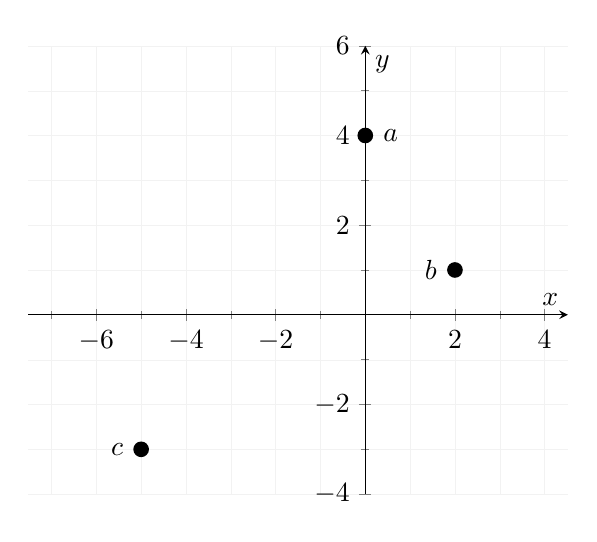
\begin{tikzpicture}
            \begin{axis}[
                    axis x line=middle, 
                    axis y line=middle, 
                    xlabel={$x$}, 
                    ylabel={$y$}, 
                    axis equal, 
                    grid=both, 
                    grid style={line width=.1pt, draw=gray!10}, 
                    minor tick num=1, 
                    ymax=6, 
                    ymin=-4
                ]

                \addplot[mark=*,only marks] coordinates {(2,1)(-5,-3)(0,4)};
                \node[label={180:{$b$}},circle,fill,inner sep=2pt] at (axis cs:2,1) {};
                \node[label={180:{$c$}},circle,fill,inner sep=2pt] at (axis cs:-5,-3) {};
                \node[label={0:{$a$}},circle,fill,inner sep=2pt] at (axis cs:0,4) {};
            \end{axis}
        \end{tikzpicture}
    \end{center}
    
    \begin{itemize}
        \item What are the coordinates of $a$? $(\answer{0},\answer{4})$
        \item What are the coordinates of $b$? $(\answer{2},\answer{1})$
        \item What are the coordinates of $c$? $(\answer{-5},\answer{-3})$
    \end{itemize}
\end{problem}


\end{document}